%---------------------------------------------------------------------------
% Gui component.
%
%---------------------------------------------------------------------------
\section{GUI component}
\label{sec:arch_gui}

Graphical user interfaces are most commonly used form of interaction with user in modern computing. Designing decent user interface is especially important due to aim of this work - creation of measurement and visualization tool. Although GUI component has rather limited role of giving user control over application and allow viewing results of the work it's in fact most complex component. Additionally any shortcoming in GUI is relatively difficult to be hidden by user, and that makes UI/UX (User Interface/User Experience) engineering so important.

While designing user interface, I've been trying to follow few general principles. First of all, I wanted resulting interface to be as transparent as possible. Users should focus on their tasks instead of learning how to use the tool. Because of that, application shouldn't be bloated with unnecessary options and steps that needs to be performed by users need to achieve their goals should be as short as possible. Because measurement visualization is probably most important functionality of application, it needs special concern. User should be able to view charts with results without any interruptions or any other UI components that might be disturbing. What is also important, GUI must be coherent to free user from chaos of being spread across multiple windows, desktops. 

From business logic point of view, GUI component will extensively use MVC design pattern\cite{gamma1995}. Each form, window or more complex section needs to have its own View, responsible for presentation, Controller that collects user's events and updates view on user actions or system events. Application will have shared model, which will be access point for underlying, external to GUI components.

\subsection{Interface Mockups}

In this section, I will try to describe mockups of most important views. First one, depicted in Figure~\ref{fig:mock_main} shows main application view. Left edge of application window contains vertical tab pane controller that will allow user to easily switch views covering most important application contexts - resources, measurements and visualizations. Another benefit of such an approach is that application has a lot of space for what user actually needs. The second most important component of main view is menu bar placed on top. It allows user to perform bulk operations (e.g. pause all measurements) regardless of view that user currently sees. 

All subsequent mockups cover context specific views that will be rendered in central pane of main view.

\begin{figure}[ht]
\centering
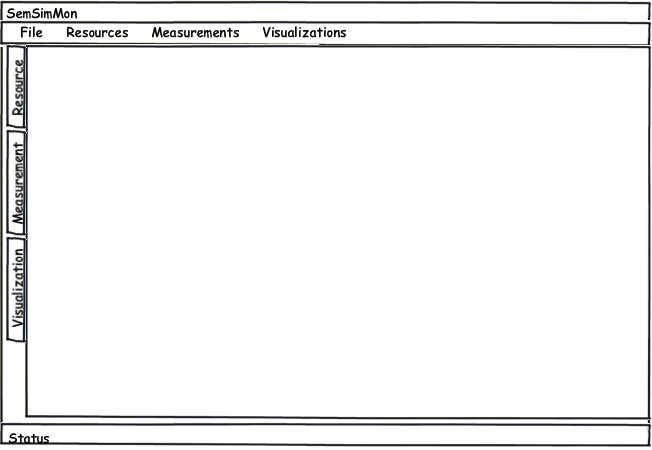
\includegraphics[width=0.7\textwidth]{mock_main}
\caption{GUI application main view mockup}
\label{fig:mock_main}
\end{figure}

When user starts working with application He or She first must add resources that will be measured. That's why resources view is first, initial section displayed directly after startup. Resources Mockup can be found in Figure~\ref{fig:mock_resources}. The view is divided into two high level logical parts - the left pane covers global resources context - users can browse measurement tree as well as add new resources into it. The right pane is specific to resource selected by user from tree on left and contains accordion with two sections. The upper one shows resource\rq{}s static attributes. The one below allows user to see snapshot of its dynamic state and check all of its capabilities at given point of time. To refresh those values, Refresh button has been provided. Additionally, below accordion there are several buttons allowing performing actions on selected resource.

\begin{figure}[ht]
\centering
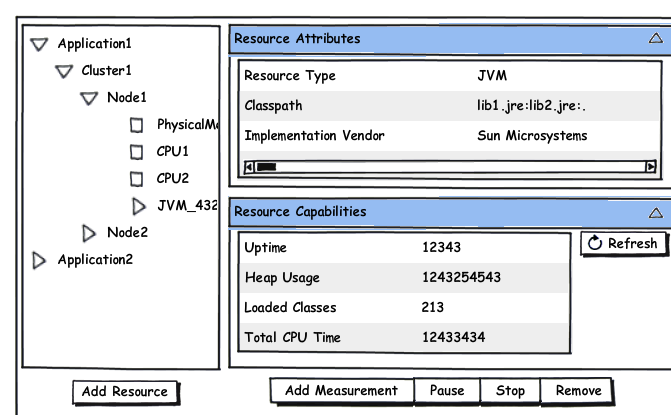
\includegraphics[width=0.7\textwidth]{mock_resources}
\caption{GUI application resources pane}
\label{fig:mock_resources}
\end{figure}

Next figure, Figure~\ref{fig:mock_measurements} covers measurements context of application. All measurements created are listed on left side of this view. After selecting one of them, accordion on the right side shows details of selected measurement. The upper section contain table with general information. The lower one shows all values gathered since creation of selected resource. Using controls under measurements list, user can pause, resume or remove measurement. Additionally in this section user may copy the results to clipboard, in CSV format which can be easily imported to any spreadsheet application for further analysis. 

\begin{figure}[ht]
\centering
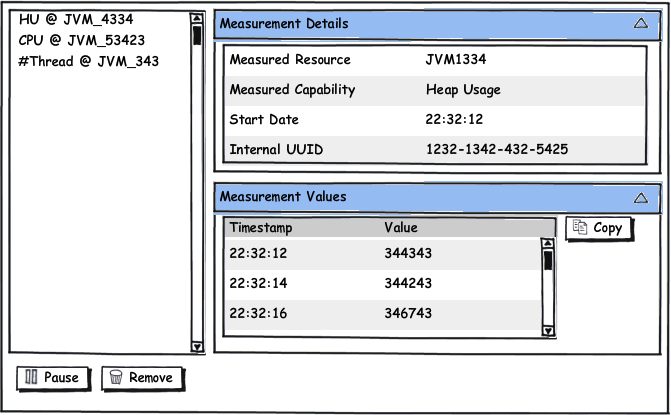
\includegraphics[width=0.7\textwidth]{mock_measurements}
\caption{GUI application measurements pane}
\label{fig:mock_measurements}
\end{figure}

\begin{figure}[ht]
\centering
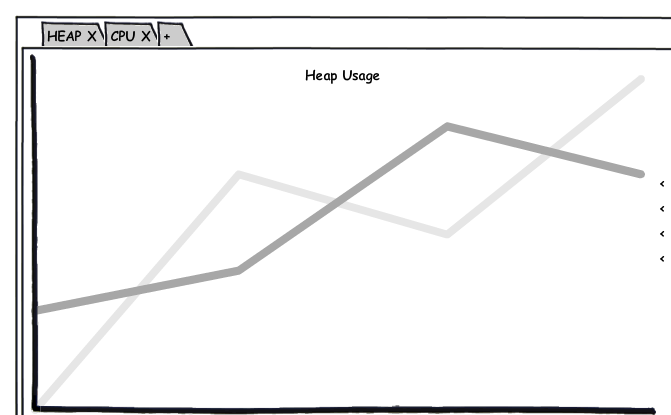
\includegraphics[width=0.7\textwidth]{mock_vis_clean}
\caption{GUI application visualizations pane, clean view}
\label{fig:mock_vis_clean}
\end{figure}

Appropriate visualizations display is probably most difficult to design from user experience engineering perspective. During designing this UI component I used modest web browsers interfaces as an inspiration. The effects can be seen in Figure~\ref{fig:mock_vis_clean} - in proposed solution every visualization is being rendered on separate, horizontal tab. To add new visualization, user should just click last tab with prompting icon. To remove visualization - user simply clicks cross icon on visualization tab - just as He or She would close tab in browser. This gives visualization chart as much space as possible and still allows user to easily control creation and disposal of visualization.

The biggest problem with such an approach is where to place controls of visualization? User must be able to choose which measurements should be included in given visualization, as well as type of chart or define other configuration settings. To address this need, management pane was designed. It is hidden by default and is being displayed to the user, on mouse over right edge of chart, marked with \lq{}<\rq{} signs. Layout of this pane is depicted in Figure~\ref{fig:mock_vis_options}. The settings pane contains form, divided into severals sections:

\begin{itemize}

\item Visualization Options - here user can configure label of whole visualization, as can be seen on tab pane

\item Chart Options - allows setting chart title (the rendered on chart graphics pane) and choose type of the chart. User will be able to use line (XY scatter), pie, bar and spider web chart types.

\item Measurements - gives control over which measurements should be included in given visualization. To add measurement into visualization, user should click Add button and from displayed dialog choose which measurements should be included. System doesn't give any constraints on measurements to be chosen, so it's up to the user to prepare reasonable visualization. User will be able to remove given measurement from chart, by simply selecting it from list and clicking Remove button.

\item Actions - allows user to pause, resume visualization. Additionally user can copy to clipboard image containing snapshot of visualization's chart.
\end{itemize}

\begin{figure}[ht]
\centering
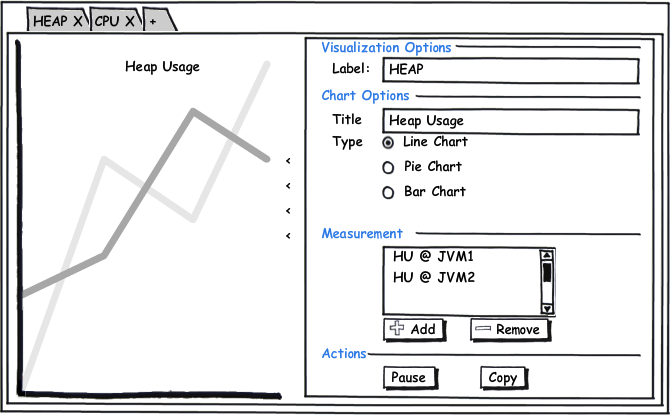
\includegraphics[width=0.7\textwidth]{mock_vis_options}
\caption{GUI application visualizations pane, view with options pane}
\label{fig:mock_vis_options}
\end{figure}

